\section{Development Method}
\label{sec:DevelopmentMethods}
In this section we will describe a few different Software development methods that we consider using.
Subsection \ref{sub:ourDevMethod} explains the method we use for this project, which is a combination of the different methods described in this section.

\subsection{Waterfall}
The waterfall method \cite{waterfallroyce}, first published by Dr. Winston W. Royce in 1970 as a flawed method of development, has derived its name directly from the concept of the method. If following this method in its traditional form, development will go through several completely separated steps, from which it is never possible to go back as seen on figure \ref{fig:WaterfallPic}. These steps will not necessarily be done by the same development teams which means that everything has to be documented thoroughly before starting the next step.

Royce originally meant for this method to be developed into a fully iterative model, however, most software development companies adapted to non-iterative form.

\begin{figure}[H]
	\centering
		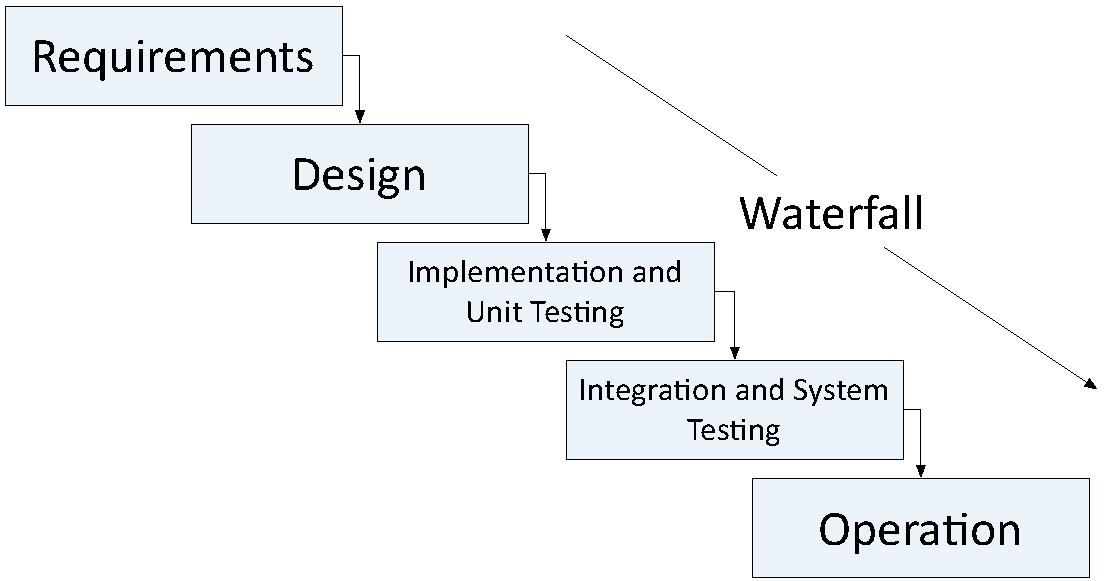
\includegraphics[width=0.90\textwidth]{input/implementation/development/waterfall.pdf}
	\morscaption{This illustrates a traditional waterfall in which the ``water'' can only proceed downwards until reaching the end (process completion)}
	\label{fig:WaterfallPic}
\end{figure}

Unfortunately, this software development method has a lot of drawbacks, the main one being its inflexibility.
Because the method is not designed to handle change in the specification during the development period, the software developed with this method could in the worst cases be useless by the time the development finishes.
Therefore it is very common for software developers to incorporate change during the development, however, because the documentation for every little piece of work has already been made at this time, it is a colossal task to change even the smallest features.
Because the changes must be made to all the documentation prior to the step where the change is made. 

\subsection{Agile Methods}
Because of the traditional and wide spread development method being so inflexible and difficult to work with, a lot of other methods is suggested.
These methods is commonly known as ``Agile'' \cite{agileManifesto}.\fixme{Mere d\ae{}kkende kilde tak.  Mvh lasse.}
In 2001 a large group formed by representatives from them most popular Agile methods came together to form ``The Agile Alliance''.
This alliance created the ``Agile Manifesto'', which states four things that the alliance think Agile Development should be:

\myQuote{
\begin{itemize}
	\item \textbf{Individuals and Interaction} over processes and tools
	\item \textbf{Working Software} over comprehensive documentation
	\item \textbf{Customer Collaboration} over contract negotiation
	\item \textbf{Responding to change} over following a plan
\end{itemize}
That is, while there is value in the items on the right, we value the items on the left more. \cite{agileManifesto}
}

\subsection{Scrum}
Scrum is an Agile development method that relies heavily on self-organizing teams. Scrum is best explained by the different components it contains:

\subsubsection{Customer / Product owner}
The customer is the person or organization for whom the development team is currently working.

\subsubsection{ScrumMaster}
The ScrumMaster is the manager of the scrum process, and is there to ensure that all developers use Scrum to achieve the maximum level of performance.

\subsubsection{Development Team}
The Development team is a set of developers working on the project. These can vary in size depending on the size of the task they have to solve.

\subsubsection{User Stories}
This is a set of stories in which the customer explains in plain language what features the product should contain, and how he/she would like them to work.

\subsubsection{Product Backlog}
This is the complete list of features -- or user stories -- that the customer would like the product to have.
Each feature is prioritized to determine the order of which these should be implemented.

\subsubsection{Sprints}
Sprints are a limited timespan, in which developers work on coding, testing and implementing the features contained in the sprint backlog.

\subsubsection{Sprint Backlog}
The Sprint backlog is the set of features that the specific development team are working on in the current sprint.

\subsubsection{Burndown Charts}
Burndown charts are the set of features that still lack implementing. Typically, a burndown chart is created for both the individual sprints and the entire project.

\subsubsection{Putting the Components Together}
When understanding all of these ``components'', one can begin to understand how they are working together to create Scrum.

The main component in Scrum is a sprint;
any sprint starts with a planning meeting in which the development team decides what features from the product backlog to work on, starting from the highest priority. 
This priority is decided by the product owner. 
When they have decided upon the features, the development team transfer them to the sprint backlog and start working.

Once a day during the sprint all team members meet with the ScrumMaster and the product owner and talk about what they have been working on the previous day, what they will be working on that day, and what might be holding them from proceeding. These meetings are held to synchronize the team members.

After completing a sprint the team demonstrates all the features added to the product. This is done to assure that the customer and the developers are on the same page.
Of course this meeting might lead to alteration of the recently implemented features, however, it might also lead to more features being added to the product backlog.

After this meeting the team starts from the top with a new planning meeting and repeat this process until the customer is satisfied with the features implemented.

\subsection{Extreme Programming (XP)}
Extreme Programming differs from the other agile methods as it is more a set of recommendations than an actual method. All sources in this subsection is from the following cites \cite{xp, xp2}.
The recommendations of XP is as following:

\subsubsection{Planning}
There are three different overall plans in XP:
\begin{itemize}
	\item \textbf{Release Planning:} The Overall plan for the project
	\item \textbf{Iteration Planning:} The plan for this iteration of development. This is very similar to the Scrum Sprints
	\item \textbf{Daily Planning:} The day to day planning between developers.
\end{itemize}
\ \\
\subsubsection{Small Releases}
This is simply about getting working software to the customer as fast as possible, better make a small release fast, than a large release slowly.

\subsubsection{Metaphor}
Find a metaphor in the real world that resembles your project.

\subsubsection{Simple Design}
Design only what you will be doing in this iteration of the project. Do not spend time designing something you might not even need later on.

\subsubsection{Testing}
The Development of the project should actually be test-driven.
That means that you write unit-tests before you write actual code.
Also, XP recommends that you run all tests simultaneously, so that you can see if a bug-correction has fixed other problems.

\subsubsection{Refactoring}
Make the code simple to modify and understand, modify existing and working code so that it is easier to modify and understand - you never know when you have to add features using or modifying existing code.

\subsubsection{Pair Programming}
In Extreme Programming one developer should never work alone. Two developers always work alongside on a single computer. XP states that this will deliver code just as quickly as two developers with two computers, however, the code will be of higher quality.

\subsubsection{Collective Ownership}
Nobody owns any code -- all code can be altered by anyone.
This is possible because unit tests for everything already exists and it allows anyone to refactor or optimize the code as long as the unit tests pass afterwards.

\subsubsection{Continuous Integration}
Always integrate the feature you have just written in the project right away.
This enhances the possibility to make a lot of small releases, and eliminates any large scale integration project at the end of development.

\subsubsection{No Overtime}
In XP projects no one should work overtime on a regular basis.
Of course it can be necessary if something in the planning slipped, however, if it becomes a regular thing something is wrong with the planning.

\subsubsection{On-Site Customer}
XP recommends that there is always a customer available, preferably on site.
This will enhance the collaboration between customer and developers and hopefully developers will not have to change as much as of the features that they have implemented.

\subsubsection{Coding Standards}
This is simply needed to implement some of the other concepts of XP, however, coding standards should not be enforced by someone higher in the company hierarchy, it should be implemented by the developers themselves.
This will be done almost by itself, as developers will grow tired of not understanding each others code.


\subsection{Development During the Project}
\label{sub:ourDevMethod}
In our project we do not strictly follow any specific development method. Instead we implement elements from scrum and extreme programming. At the start of each day we hold a meeting to discuss what we will be doing during the day. Furthermore we have a lot of small sprints, where we focus on developing, integrating and testing new features. These sprints are very short, typically maximum a couple of days, because our development phase do not last for more than a couple of weeks.

Beside the principles borrowed from scrum, we also uses a lot of elements from Extreme Programming:
\begin{itemize}
\item We plan our project in a similar way to XP
\item We are constantly been making small releases 
\item We write a release every time we have developed/implemented a new feature
\item We have collective ownership of all our code
\item We write tests for all our major components 
\item We are continuously integrating the created features into our main application
\item We do not have regular overtime in this project.
\item We try to maintain coding standards.
\end{itemize}
\fixme{ret kilder - der er 2 ``Scrum''}
Using these elements it much easier for us to delegate our work and plan all the aspects of our project. Also, it has given us a all a better understanding of our code, as all collaborates to achieve our goal, and often edites each others' code. The swift development of our application and the fact we almost never work late has helped us to maintain a high interest in the project.